\documentclass[a4paper,12pt]{article}
\title{MATH1106 DIS207/208 Practice Quiz 2 Solutions}
\author{Benjamin Thompson}
\date{February 26, 2020}

\usepackage[margin=1in]{geometry}

\usepackage{hyperref}
\usepackage{amsmath}
\usepackage[usenames,dvipsnames]{xcolor}
\usepackage{tikz}
\usetikzlibrary{arrows.meta,decorations.markings}


\usepackage{pgfplots}

\pgfplotsset{every axis/.append style={
axis x line=middle,    % put the x axis in the middle
axis y line=middle,    % put the y axis in the middle
axis line style={-{Stealth[length=3mm]},color=black}, % arrows on the axis
minor tick num=1
            }}


\usepackage{fancyhdr}
\pagestyle{fancy}

\fancyhf{}
\lhead{MATH1106 DIS207/208 Practice Quiz 2 Solutions}
\rhead{February 26, 2020}
\cfoot{\thepage}

\usepackage{enumitem}

\newcommand{\bfa}{\mathbf{a}}
\newcommand{\bfb}{\mathbf{b}}
\newcommand{\bfc}{\mathbf{c}}
\newcommand{\bfd}{\mathbf{d}}


\begin{document}
\subsubsection*{Name:}
Each of the multiple choice questions below has one correct choice. Circle the correct choice. (NOTE: The quiz presented in class had errors in Q1 and Q2, these have been corrected.)
\subsubsection*{Q1}
An SIR model of an epidemic is created and described by the following differential equations, where $A$, $B$, $C$ represent susceptible, infectious, and recovered populations, but not necessarily in that order.
\begin{align*}
A' &= \gamma C \\
B' &= -\beta BC  \\
C' &= \beta BC - \gamma C
\end{align*}
A vaccine is developed, and the model is updated to incorporate this change. Assuming that vaccinated individuals are immune from the disease and are not infectious, which of the following is a change equation in the new model?

\begin{enumerate}[label=(\alph*)]
\item $A' = \gamma C - \delta A$
\item $B' = -\beta BC - \delta B$
\item $C' = \beta BC - \gamma A - \delta A$
\item $C' = \beta BC - \gamma A + \delta A$
\end{enumerate}

\textbf{Solution:} \emph{The equations describe the SIR model without vital dynamics. (See for instance, the Wikipedia page on the SIR model.\footnote{Section 2.1 at \url{https://en.wikipedia.org/wiki/Compartmental_models_in_epidemiology}}) This is the simplest version of the model, where there are no births or deaths, just transmission. Before vaccination is added, the only possible transition for susceptible individuals is to infectious, which requires an encounter. The only equation fitting these criteria is $B' = -\beta BC$, so $B = S$, and hence $C = I$. By elimination we then have $R = A$. The change equation for $A$ implies that recovered individuals cannot get infected again, so we can model vaccination as a process taking susceptible individuals to recovered individuals. The would mean adding a $-\delta S$ term to $S'$ or a $+\delta S$ term to $R$. As $S = B$, this means the change equation for $B$ should be $B' = -\beta BC - \delta B$, which is option \textbf{(b)}}.
\subsubsection*{Q2}
Recall the Romeo and Juliet model given by the change equations
\begin{align*}
	J' &= R \\
	R' &= -J.
\end{align*}
Which of the following statements regarding the vector field of the model is false?
\begin{enumerate}[label=(\alph*)]
\item If the vector field is rotated by $180^{\circ}$ around the origin, the rotated vector field is identical to original vector field.
\item The length of a vector at a point $(A,A)$ is $|A|\sqrt{2}$.
\item Only one vector in the vector field has length $0$.
\item Vectors at different points have different directions.
\end{enumerate}
\textbf{Solution: } \emph{The Romeo and Juliet model has been covered several times, the vector field essentially has circular trajectories. This can be seen by using plotting software to graph the vector field, e.g. using Desmos. NOTE: this is an essential skill, if you don't know how to use at least one piece of software to plot a simple vector field please reach out to friends for help or ask about it in office hours. In such a plot it is clear visually that the vector field has rotational symmetry about the origin, so (a) is true. The vector at the point $(A,A)$ is $(A,-A)$, which has length $\sqrt{A^2 + (-A)^2} = \sqrt{2A^2} = |A|\sqrt{2}$. (Here $|x|$ denotes the absolute value of a number. NOTE: This is also essential, check up the definition on Wikipedia if you don't know it.) So (b) is also correct. Note that the vectors at the points $(1,0)$ and $(2,0)$ are $(0,-1)$ and $(0,-2)$ respectively, which have the same direction. As such, there are some vectors at different points which have the same direction, so \textbf{(d)} is false.}
\subsubsection*{Q3}
The growth of a certain protozoa population is found to be described by
\[
	P' = \sqrt{P} + 4.
\]
At time $t=100$ the population is $9$. Euler's method is used to estimate the population at time $t=102$ using the interval $\Delta t = 1$. This estimate is:

\begin{enumerate}[label=(\alph*)]
\item $4 + \sqrt{7}$
\item $16$
\item $24$
\item $18 + \sqrt{14}$
\end{enumerate}

\textbf{Solution:} \emph{Applying Euler's method with $\Delta t = 1$ will compute $P$ at $t=101$, and then at $t=102$, at which point we can stop. When $t=100$, $P' = \sqrt{9} + 4 = 7$, so $P$ at $t=101$ is given by $P + \Delta T \cdot P' = 9 + 1 \cdot 7 = 16$. When $t=101$, we then have $P' = \sqrt{16} + 4 = 8$, so $P$ at $t=102$ is given by $P + \Delta \cdot P' = 16 + 1 \cdot 8 = 24$, hence \textbf{(c)}.}

\subsubsection*{Q4}
A line in the $xy$-plane has passes through the points $(2,0)$ and $(0,1)$. The line has slope:
\begin{enumerate}[label=(\alph*)]
\item $-2$
\item $2$
\item $-\frac{1}{2}$
\item $\frac{1}{2}$
\end{enumerate}

\textbf{Solution:} \emph{The slope of a line is defined as the rise / run, or, given any two points on the line, the change in $y$ between the points divided by the change in $x$ between the points. As such we have}
\[
	\text{slope} = \frac{0 - 1}{2 - 0} = -\frac{1}{2},
\]
\emph{hence \textbf{(c)}.}

\subsubsection*{Q5}
The state space trajectory of a system with variables $M$, $N$ is shown below. Assuming that as time increases \emph{the trajectory goes in a clockwise direction}, which of the following graphs is a possible time-series of the trajectory? (Note: in the time-series graphs, the horizontal axis represents time.)
\[
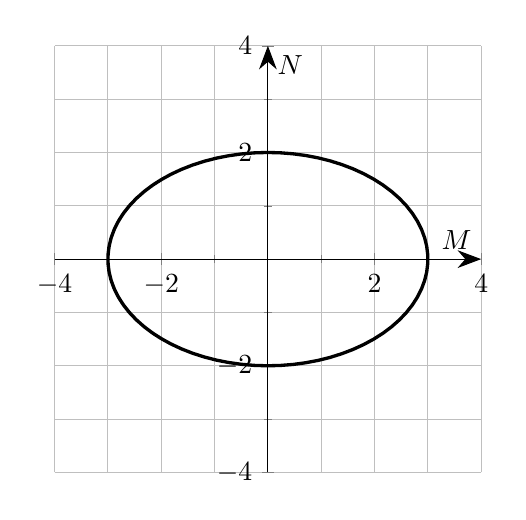
\begin{tikzpicture}
\begin{axis}[xlabel={$M$},ylabel={$N$},width=7cm, height=7cm, xmin=-4,xmax=4, ymin=-4,ymax=4, grid=both]
\addplot [very thick, domain=-4:4,samples=100]({3*cos(deg(x))},{2*sin(deg(x))}); 
\end{axis}
\end{tikzpicture}
\]
\[
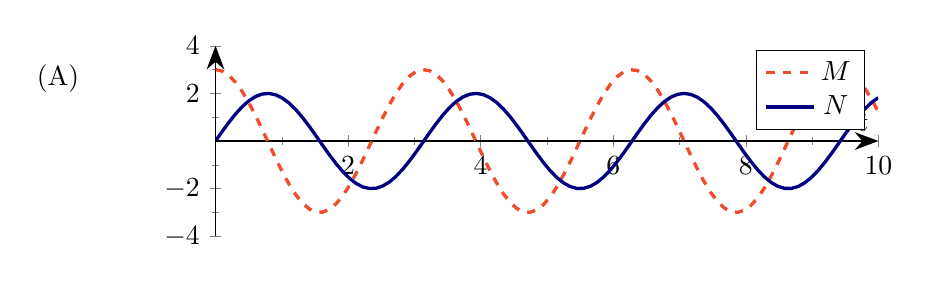
\begin{tikzpicture}

\begin{axis}[xlabel={$t$},width=10cm, height=4cm, xmin=0,xmax=10, ymin=-4,ymax=4, grid=none]
\addplot [dashed,RedOrange,very thick,domain=0:10,samples=100]{3*cos(2*deg(x))};
\addlegendentry{$M$}
\addplot [NavyBlue,very thick, domain=0:10,samples=100]{2*sin(2*deg(x))}; 
\addlegendentry{$N$}
\end{axis}

\node (A) at (-2,2) {(A)};
\end{tikzpicture}
\]
\[
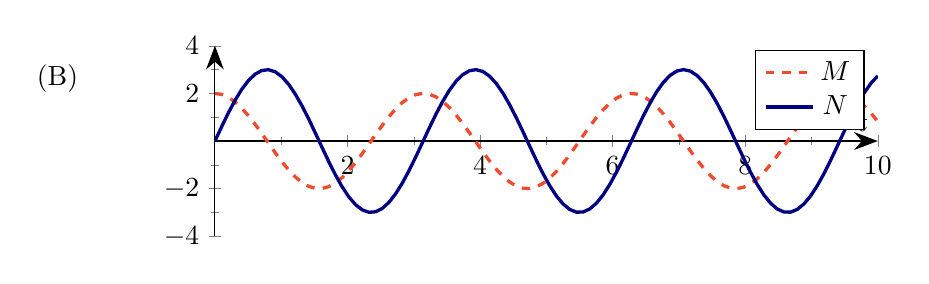
\begin{tikzpicture}

\begin{axis}[xlabel={$t$},width=10cm, height=4cm, xmin=0,xmax=10, ymin=-4,ymax=4, grid=none]
\addplot [dashed,RedOrange,very thick,domain=0:10,samples=100]{2*cos(2*deg(x))};
\addlegendentry{$M$}
\addplot [NavyBlue,very thick, domain=0:10,samples=100]{3*sin(2*deg(x))}; 
\addlegendentry{$N$}
\end{axis}

\node (B) at (-2,2) {(B)};
\end{tikzpicture}
\]
\[
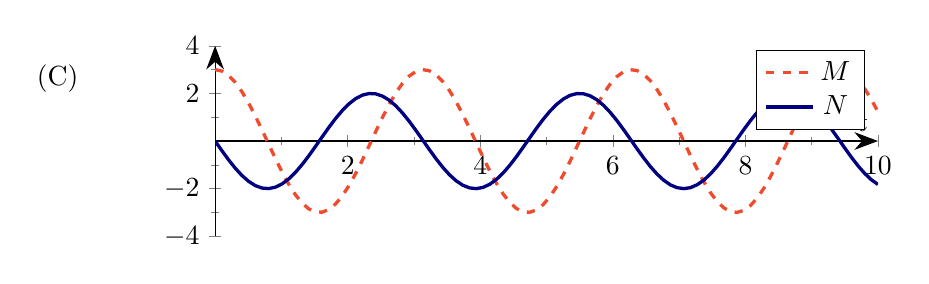
\begin{tikzpicture}

\begin{axis}[xlabel={$t$},width=10cm, height=4cm, xmin=0,xmax=10, ymin=-4,ymax=4, grid=none]
\addplot [dashed,RedOrange,very thick,domain=0:10,samples=100]{3*cos(2*deg(x))};
\addlegendentry{$M$}
\addplot [NavyBlue,very thick, domain=0:10,samples=100]{-2*sin(2*deg(x))}; 
\addlegendentry{$N$}
\end{axis}

\node (C) at (-2,2) {(C)};
\end{tikzpicture}
\]
\[
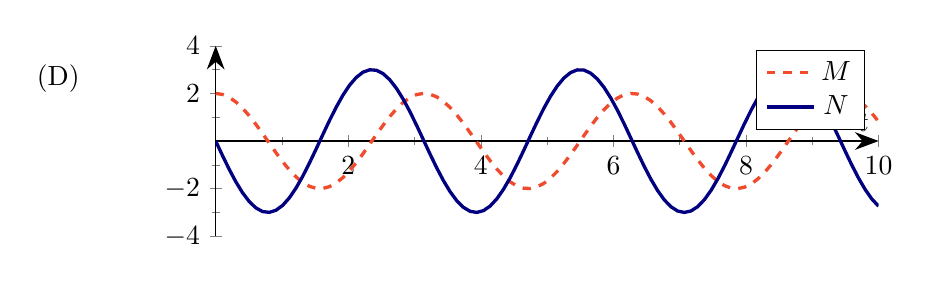
\begin{tikzpicture}

\begin{axis}[xlabel={$t$},width=10cm, height=4cm, xmin=0,xmax=10, ymin=-4,ymax=4, grid=none]
\addplot [dashed, RedOrange,very thick,domain=0:10,samples=100]{2*cos(2*deg(x))};
\addlegendentry{$M$}
\addplot [NavyBlue,very thick, domain=0:10,samples=100]{-3*sin(2*deg(x))}; 
\addlegendentry{$N$}
\end{axis}

\node (D) at (-2,2) {(D)};
\end{tikzpicture}
\]

\textbf{Solution:} \emph{This may look scary, but it's not too bad. We can read off from the trajectory that the range of possible $N$ values is the interval $[-2,2]$, and the range of possible $M$ values is $[-3,3]$. As such, in the time series the peaks of $M$ should be higher than the peaks of $N$. This immediately rules out options (B) and (D).}

\emph{To choose between the remaining options, choose a point on the trajectory, and consider a point close to it moving clockwise. Peaks are easy to work with, so consider the most vertical point in the trajectory plot. This is at a peak of $N$. As the trajectory moves clockwise, the value of $M$ increases. This should be reflected in the graphs.}

\emph{Examining the peaks of $N$ in graph (A), we see that after them $M$ is decreasing, so by elimination the solution is \textbf{(C)}. (And indeed, in (C), directly after $N$ peaks, $M$ increases.)}
\end{document}
